\documentclass{beamer}
\usepackage[utf8]{inputenc}
\usepackage[backend=biber,style=ieee]{biblatex}
\addbibresource{Project 460.bib}
\usetheme{Madrid}
\usecolortheme{default}
%------------------------
%------------------------------------
%This block of code defines the information to appear in the
%Title page
\title[SSALD] %optional
{Semi-Supervised Active Learning Guided Detection System (SSALD)}

\subtitle{Mid-way deliverables for CS-460}

\author[] % (optional)
{Aniket Nath\inst{1}\inst{2} \and Diptarko Choudhury\inst{1}\inst{2}}

\institute[NISER] % (optional)
{
	\inst{1}%
	School of Physical Sciences\\
	National Institute of Science Education and Research, HBNI
	\and
	\inst{2}%
	School of Computer Sciences\\
	National Institute of Science Education and Research, HBNI

}

\date[\today] % (optional)
{\today}

\logo{
\includegraphics[height=1cm]{logo_niser.png}}

%End of title page configuration block
%------------------------------------------------------------



%------------------------------------------------------------
%The next block of commands puts the table of contents at the 
%beginning of each section and highlights the current section:


%------------------------------------------------------------

\begin{document}
	
	%The next statement creates the title page.
	\frame{\titlepage}
	
	
	%---------------------------------------------------------
	%This block of code is for the table of contents after
	%the title page
	\begin{frame}
		\frametitle{Table of Contents}
		\tableofcontents
	\end{frame}
	%---------------------------------------------------------
	
	
\section{Introduction}
\begin{frame}[allowframebreaks]{Introduction}{Problem Statement}
	In our low redshift universe, the main mechanism for growth of galaxies is through mergers of galaxies [7]. Galaxies usually have a Super Massive Black Hole (SMBH) , at it's center, which provides the gravitational potential for the substructures to form. When two galaxies merge, their nuclear bulge hosting the SMBH, come closer and interact with each other, forming dual or even in certain cases multiple nuclei galaxies. Often, merger process triggers accretion disk around the SMBHs, leading to the formation of an Active Galactic Nuclei (AGN) [5].
	\begin{figure}
		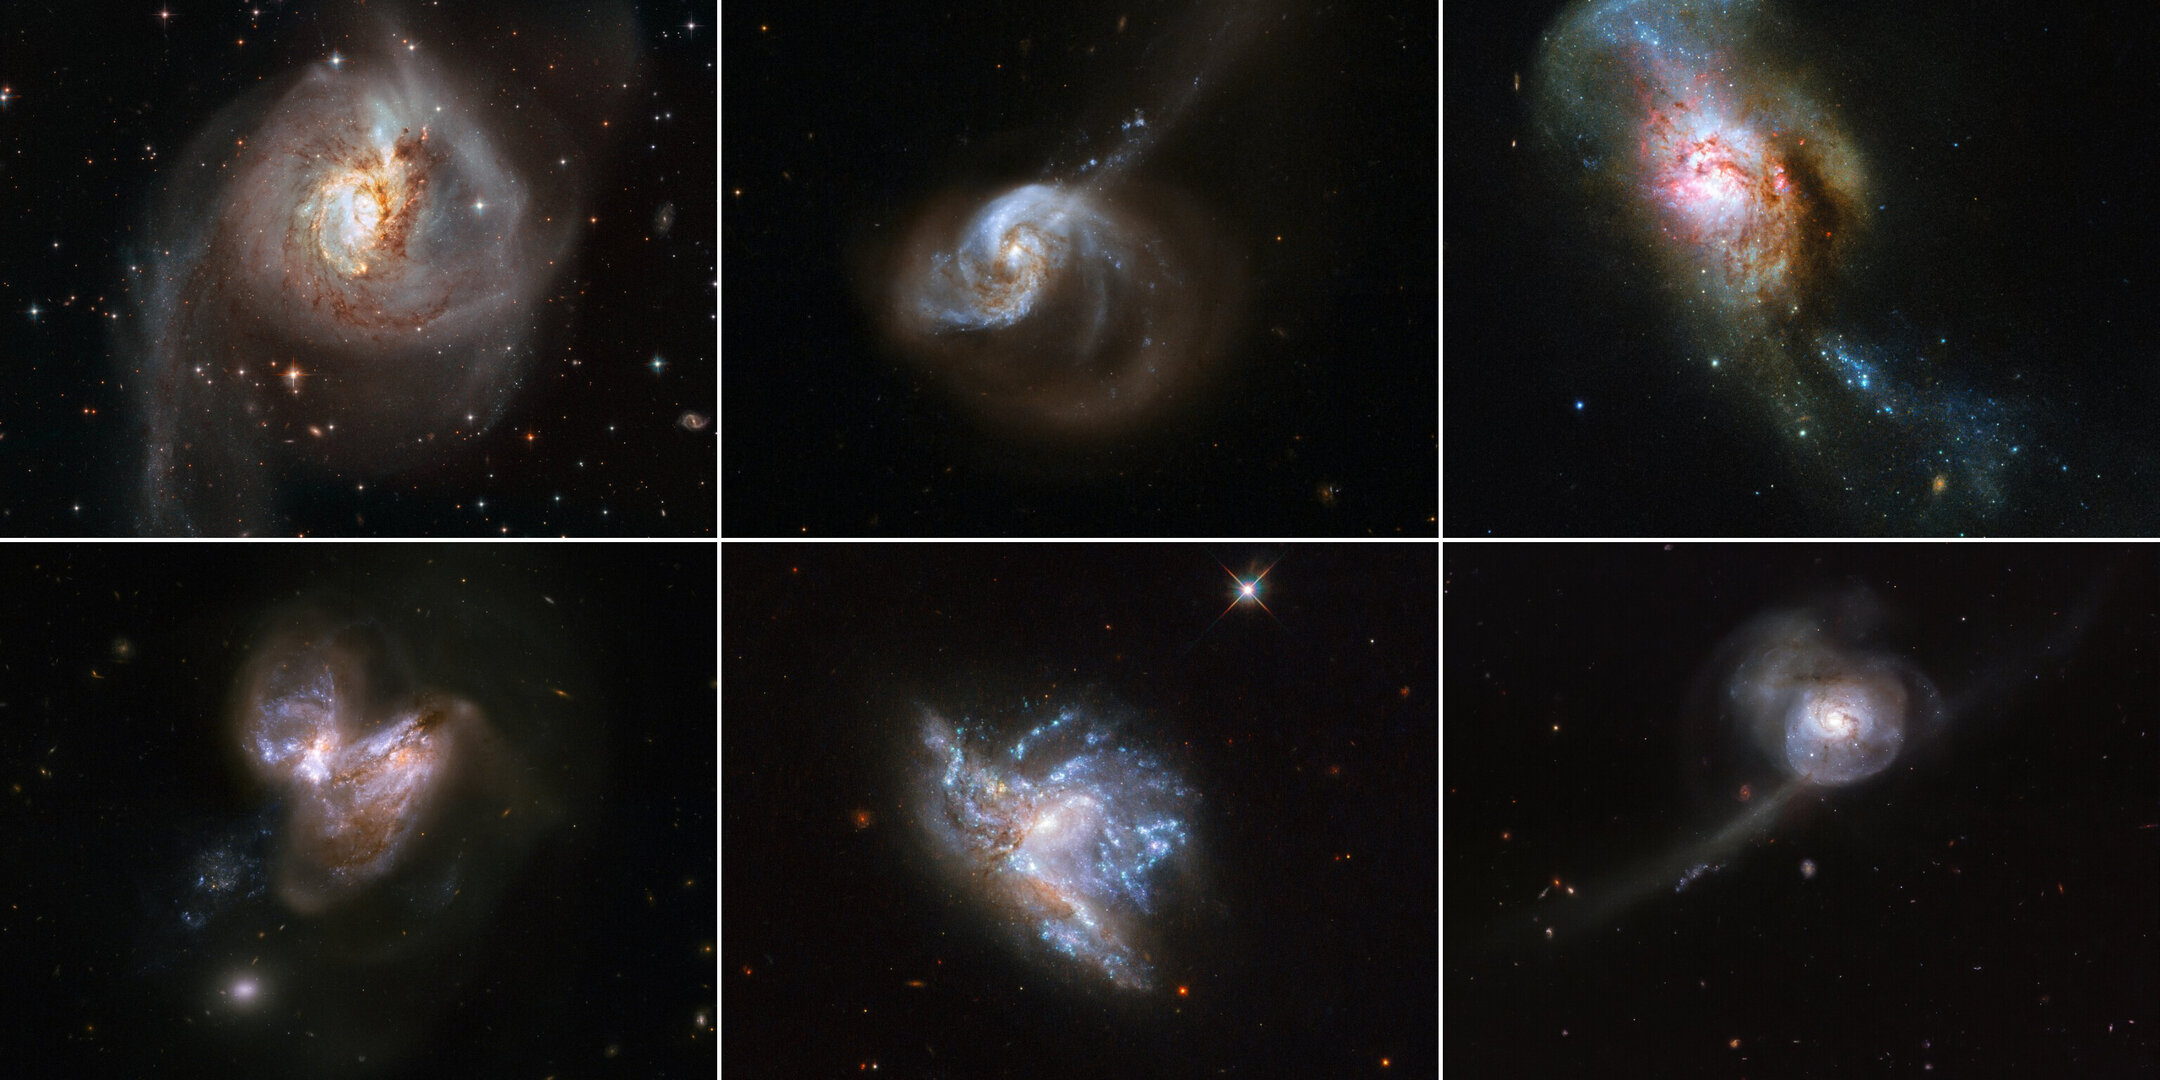
\includegraphics[scale=0.15]{mergers.jpg}
		\caption{Images of Galaxy Mergers taken from ESA Hubble Space Telescope [?]}
	\end{figure}
\end{frame}
\section{Methodology}
\begin{frame}{Methodology}{Steps}
	We aim to use an Active Learning guided self-supervised algorithm to solve our problem. In the
	following sections, we discuss our strategy in a step-by-step fashion.
	\begin{itemize}
		\item Supervised Learning
		\item Unsupervised and Semi-Supervised Learning
		\item Self-Supervised Learning
		\item Active Learning
	\end{itemize}
\end{frame}
\begin{frame}{VICReg}
	\begin{figure}
		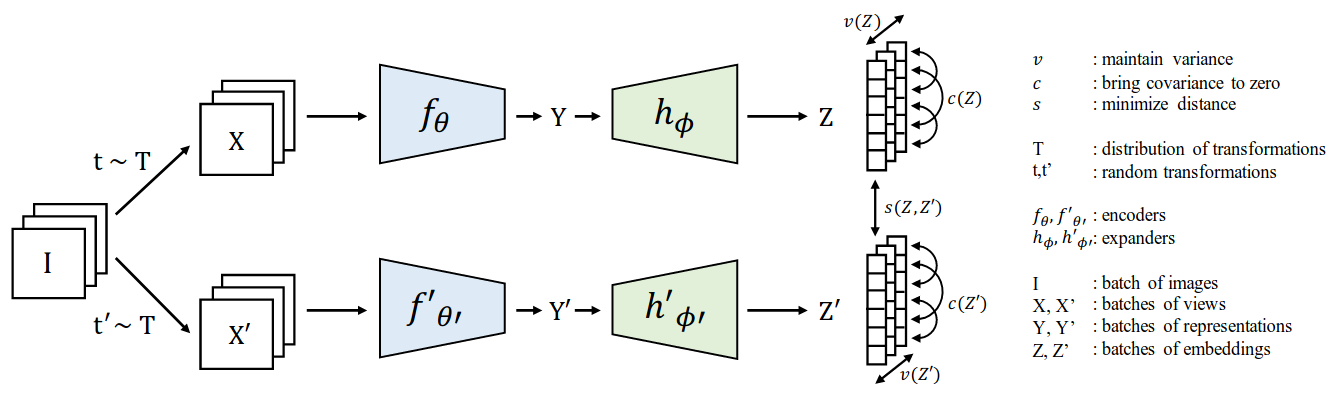
\includegraphics[scale=0.25]{VICReg.png}
		\caption{Schematics of VICReg Algorithm [6]}
	\end{figure}

\end{frame}

\section{Related Works}
\begin{frame}{Related Works}
	\begin{itemize}
		\item GOTHIC
		\item Hayat et. al.
	\end{itemize}
\end{frame}
\section{Results}
\begin{frame}
	\frametitle{Results}
	content...
\end{frame}
\section{Conclusion}
\begin{frame}
	\frametitle{Conclusion}
	content...
\end{frame}
\begin{frame}{References}

	\printbibliography
\end{frame}
	%---------------------------------------------------------
	
	
\end{document}